\documentclass{article}
\usepackage[T1]{fontenc}
\usepackage{lmodern}
\usepackage{graphicx}
\usepackage{amsmath,amssymb}
\usepackage[a4paper,margin=2cm]{geometry}
\usepackage[absolute,overlay]{textpos}
\setlength{\TPHorizModule}{1mm}
\setlength{\TPVertModule}{1mm}
\usepackage[indonesian]{babel}
\usepackage{hyperref}
\setlength{\emergencystretch}{2em}
% unit: Halaman 27

\begin{document}

% === Halaman 27 (llm) ===

\vspace{241.16mm}

Cipherteks: VIVBQ SQBI SMBMUC LQ ICTI

% deskripsi: Tabel pergeseran kunci k dari 0 sampai 25 dengan hasil dekripsi teks cipher. Baris k=8 ditandai tebal dengan teks 'nanti kita ketemu di aula'.
% bbox normalisasi: [0.2200, 0.1300, 0.6080, 0.9420]
\begin{textblock*}{81.48mm}(46.20mm,38.61mm)
\noindent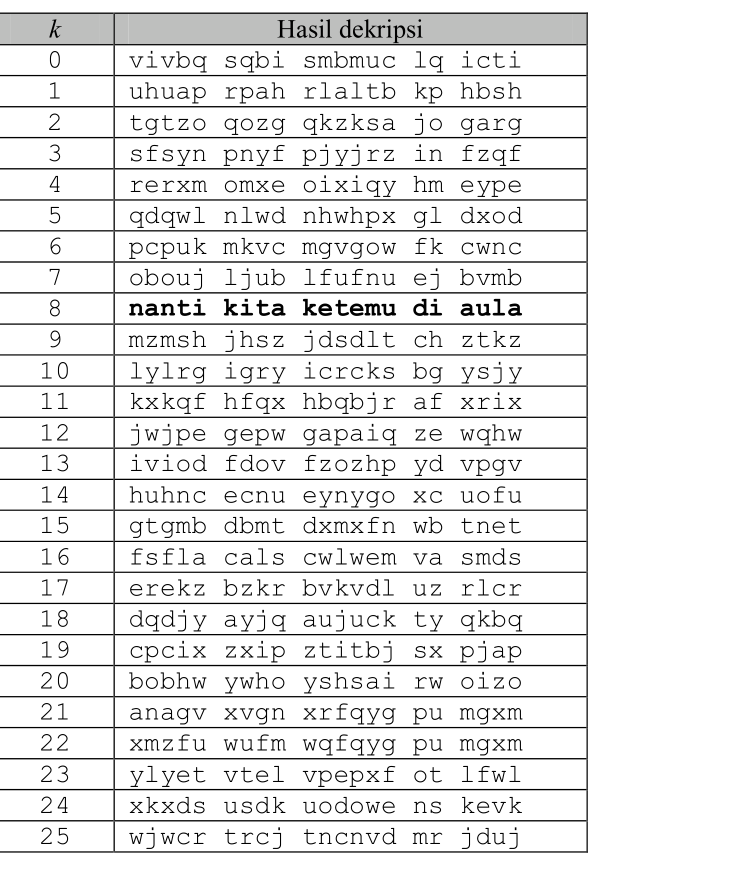
\includegraphics[width=81.48mm,height=241.16mm]{../../images/llm/page_027_img_01.png}%
\end{textblock*}

\end{document}
